\documentclass[aspectratio=169, 14pt]{beamer}
\usepackage[utf8]{inputenc}
\usepackage{xeCJK}
\usepackage{graphicx}
\usepackage{transparent}
\usepackage{amsmath}
\usepackage[ruled, lined, linesnumbered, commentsnumbered]{algorithm2e}
\usepackage{pgfplots}
\usepackage{tikz}
\usetikzlibrary{matrix,backgrounds}
\usetikzlibrary{arrows}
\usetikzlibrary {arrows.meta}
\usetikzlibrary{calc,shadows.blur,fit,positioning}
\usepackage{minted}
\usepackage{fontawesome5}
\usepackage{booktabs}
\usepackage{caption}
\usepackage{hyperref}
\hypersetup{
    colorlinks=true,
    linkcolor=blue,
    filecolor=magenta,      
    urlcolor=cyan,
    }
\urlstyle{same}
\usetheme{metropolis}
\metroset{block=fill}
\usecolortheme{default}
\definecolor{darkmidnightblue}{rgb}{0.0, 0.2, 0.4}
\definecolor{LightGray}{gray}{0.9}


%------------------------------------------------------------
%This block of code defines the information to appear in the
%Title page
\title[Database Principles and Applications] %optional
{数据库原理与应用}

\subtitle{SQL Lab}

\author[CHEN Zhongpu] % (optional)
{CHEN Zhongpu}

\institute[] % (optional)
{
  School of Computing and Artificial Intelligence \\
  \href{mailto:zpchen@swufe.edu.cn}{zpchen@swufe.edu.cn}
}

\date[] % (optional)
{SWUFE, Fall 2022}

%End of title page configuration block
%------------------------------------------------------------


%------------------------------------------------------------
%The next block of commands puts the table of contents at the 
%beginning of each section and highlights the current section:

% \AtBeginSection[]
% {
%   \begin{frame}
%     \frametitle{Table of Contents}
%     \tableofcontents[currentsection]
%   \end{frame}
% }
%------------------------------------------------------------


\begin{document}

%The next statement creates the title page.
\frame{\titlepage}

%---------------------------------------------------------
%This block of code is for the table of contents after
%the title page
% \begin{frame}
% \frametitle{Table of Contents}
% \tableofcontents
% \end{frame}
%--------------------------------------------------------
\begin{frame}
    \frametitle{复习}
    \begin{enumerate}
        \item 基本类型(数、字符串)
        \item 定义关系(\texttt{create table})
        \item 查询关系(\texttt{select}, \texttt{from}, \texttt{where})
        \item 更名运算(\texttt{as})、排序子句(\texttt{order by})    
    \end{enumerate}
\end{frame}

{
    % \usebackgroundtemplate{\transparent{0.3}{\begin{picture}
    %     
\includegraphics[height=0.7\paperheight]{cover}
    % \end{picture}    
    % }}
\usebackgroundtemplate{
  \tikz[overlay,remember picture] 
  \node[opacity=0.3, at=(current page.south east),anchor=south east, yshift=2cm,xshift=4cm] {
    
\includegraphics[height=0.6\paperheight]{cover}};
}
    \begin{frame}
        \section{\textcolor{darkmidnightblue}{1. 环境搭建}}
    \end{frame}
}


\begin{frame}
    \frametitle{1.1 PostgreSQL: MacOS}
    安装\href{https://postgresapp.com/}{Postgres.app}。

    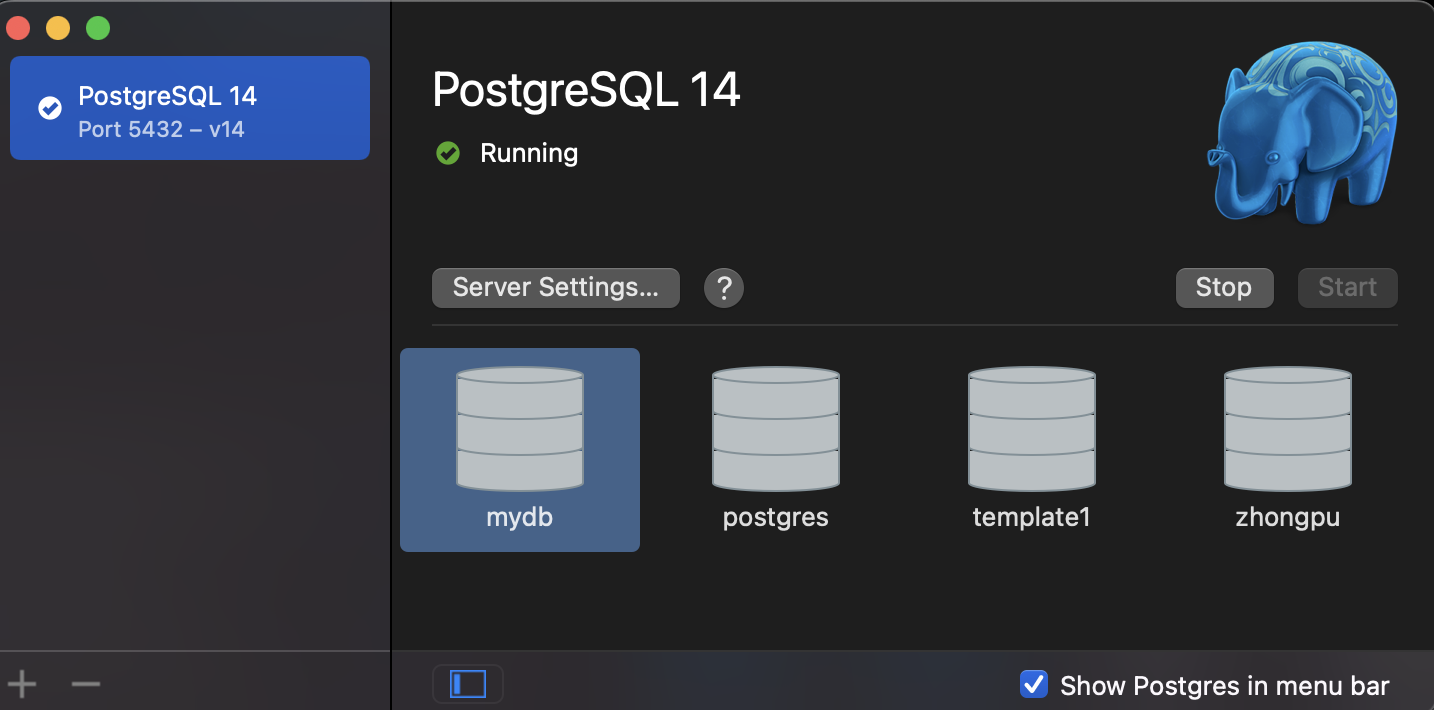
\includegraphics[width=.8\textwidth]{week4/pg-mac}

\end{frame}

\begin{frame}[fragile]
    \frametitle{MacOS:新建数据库}
    
    打开终端(terminal),输入

    \begin{minted}[bgcolor=LightGray]{shell}
createdb mydb
    \end{minted}

成功后,并没有任何提示,但能从Postgres.app软件中可见。
\end{frame}

\begin{frame}
    \frametitle{1.2 PostgreSQL: Windows}
    在所有程序中,PostgreSQL $\rightarrow$ SQLShell:

    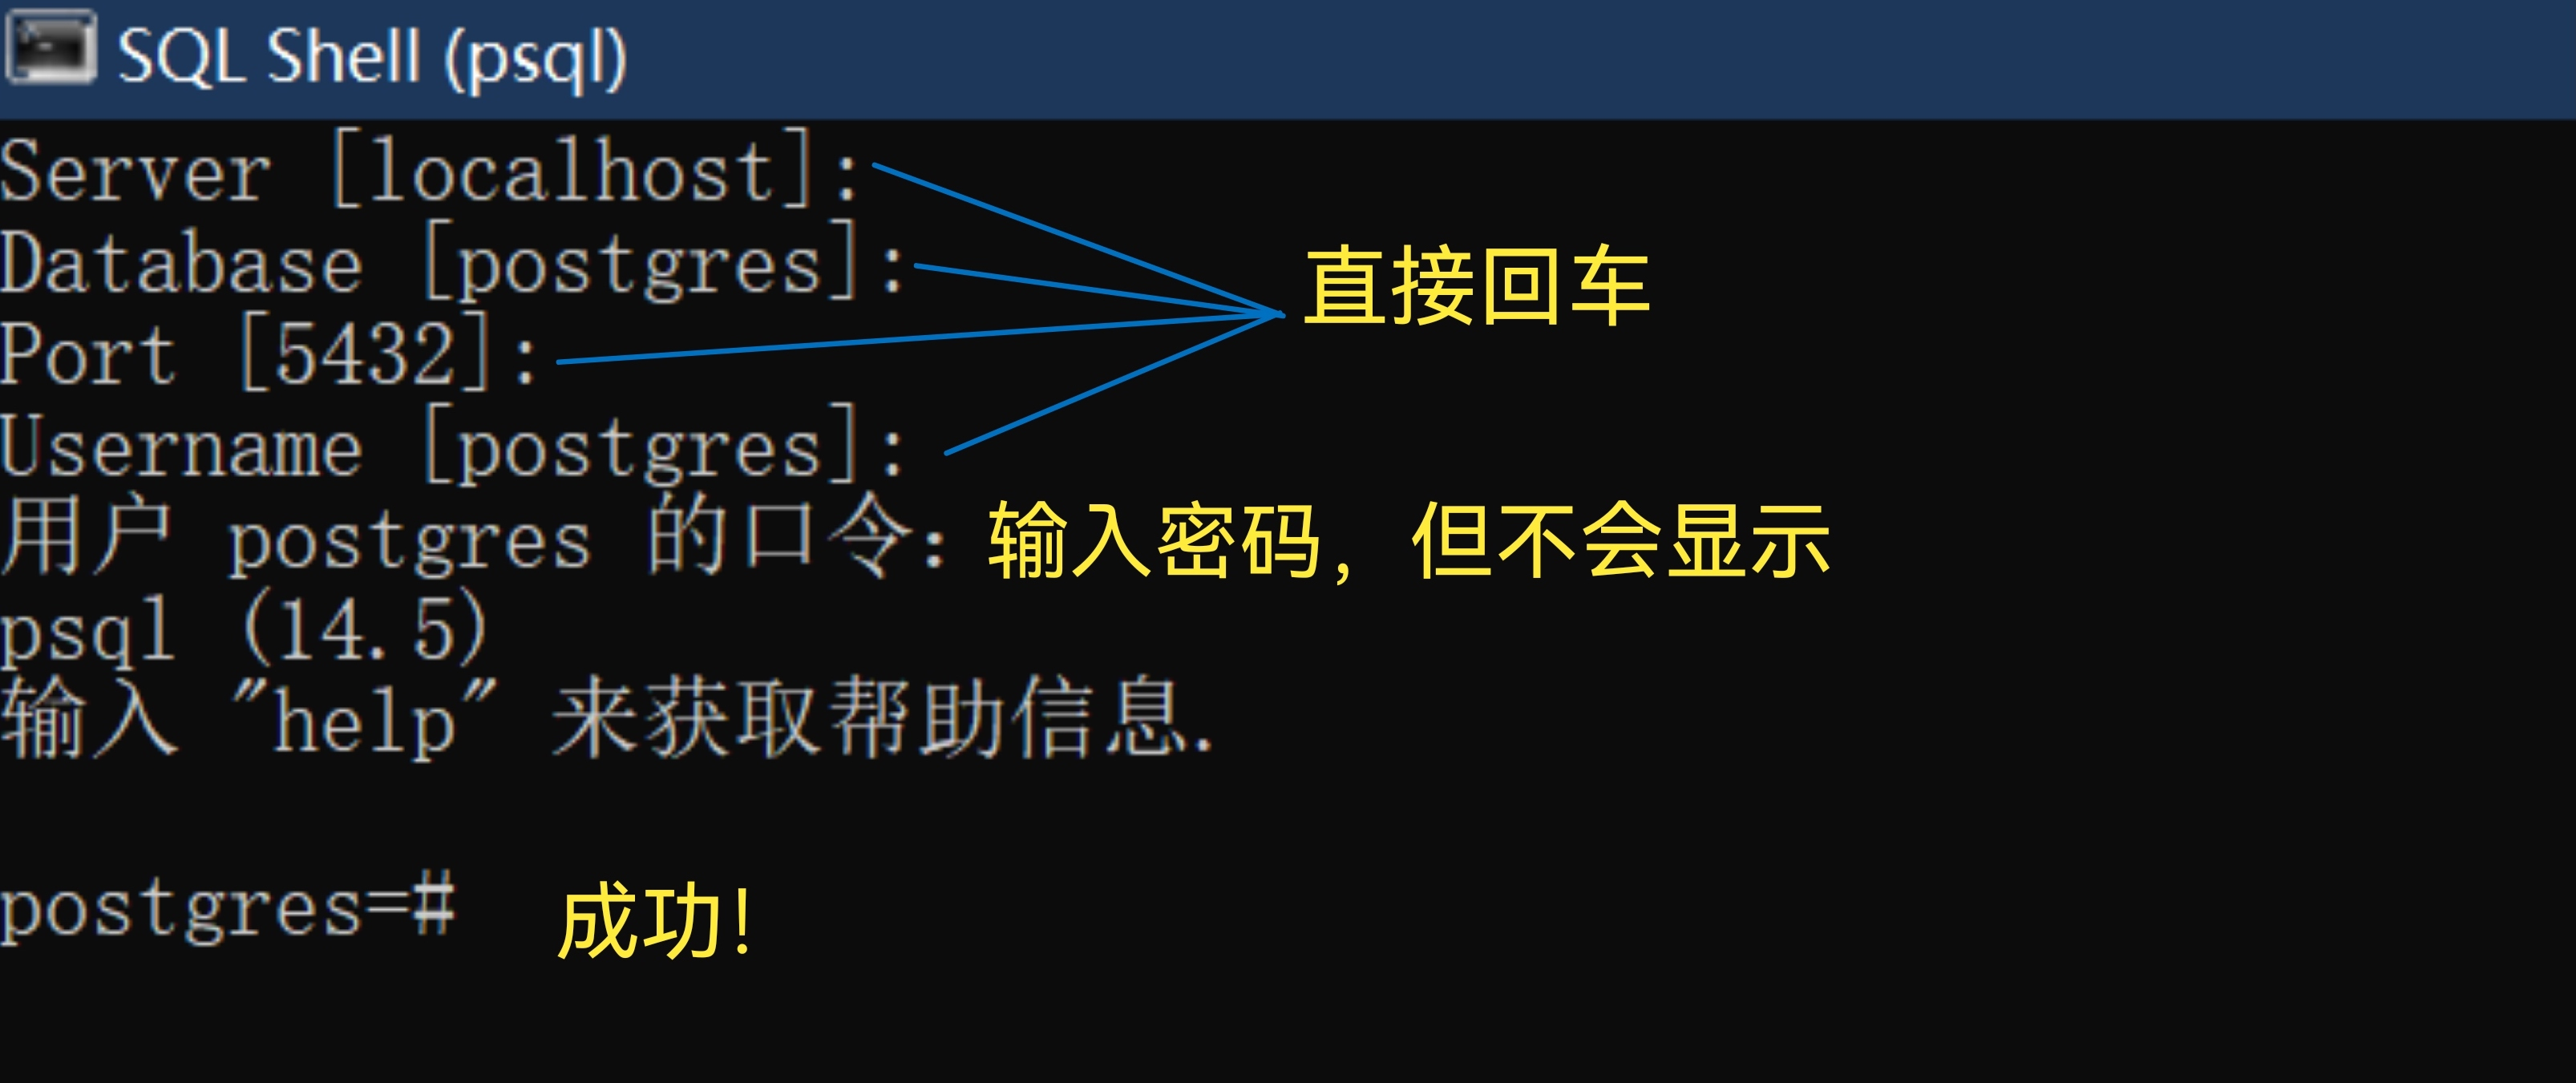
\includegraphics[width=.8\textwidth]{week4/pg-windows}
\end{frame}

\begin{frame}[fragile]
    \frametitle{Windows:新建数据库}
在上述psql终端中(在\texttt{postgres=\#}后面),输入:

\begin{minted}[bgcolor=LightGray]{sql}
CREATE DATABASE mydb; 
\end{minted}

注意,需要以分号结尾。
\end{frame}

\begin{frame}
    \frametitle{1.3 新建工程}
打开DataGrip,点击「New Project」:

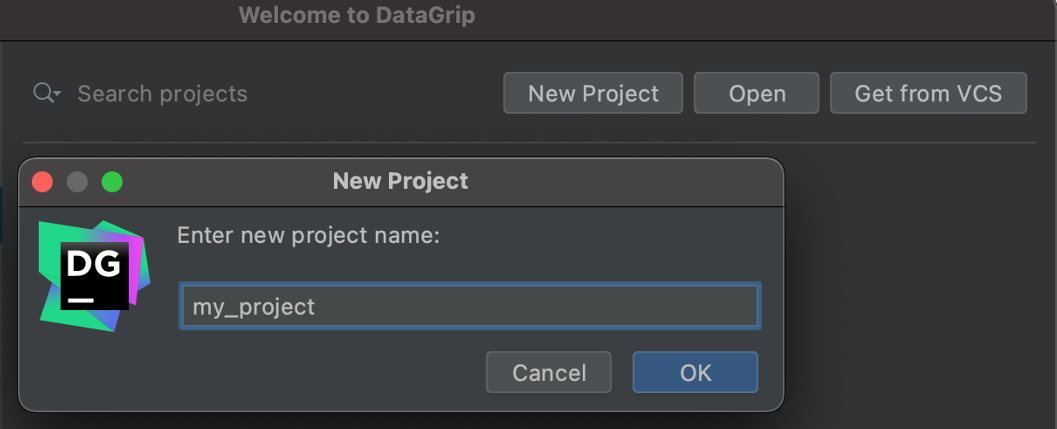
\includegraphics[width=.8\textwidth]{week4/welcome}

\end{frame}

\begin{frame}
    \frametitle{1.4 连接数据库} 
    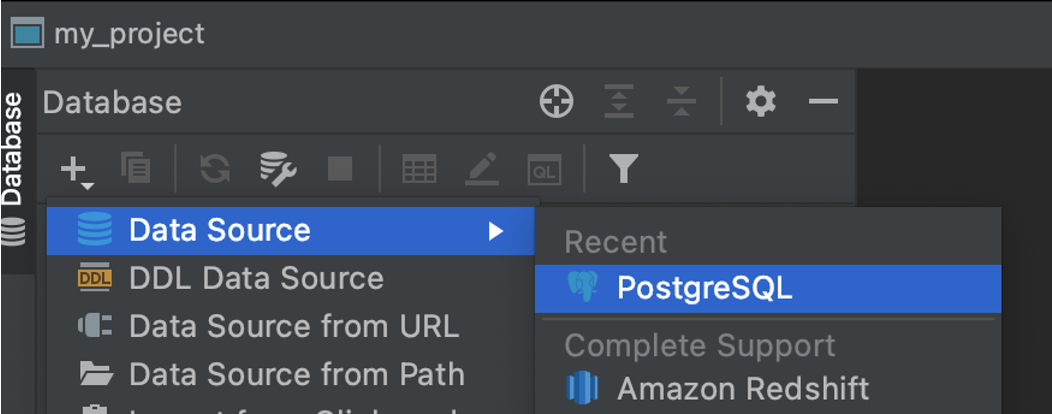
\includegraphics[width=.8\textwidth]{week4/datasource}

    或者点击 File $\rightarrow$ New $\rightarrow$ Data Source $\rightarrow$ PostgreSQL

    \begin{tikzpicture}
        \node[fill=yellow,blur shadow={shadow xshift=-0.5ex},
        text width=23em,anchor=south west,rounded corners]
        {第一次使用会出现「missing driver files」的提示,点击旁边的「Download」即可};
    \end{tikzpicture}
\end{frame}

\begin{frame}
确保 User 是 \alert{postgres},Database 是 \alert{mydb}:

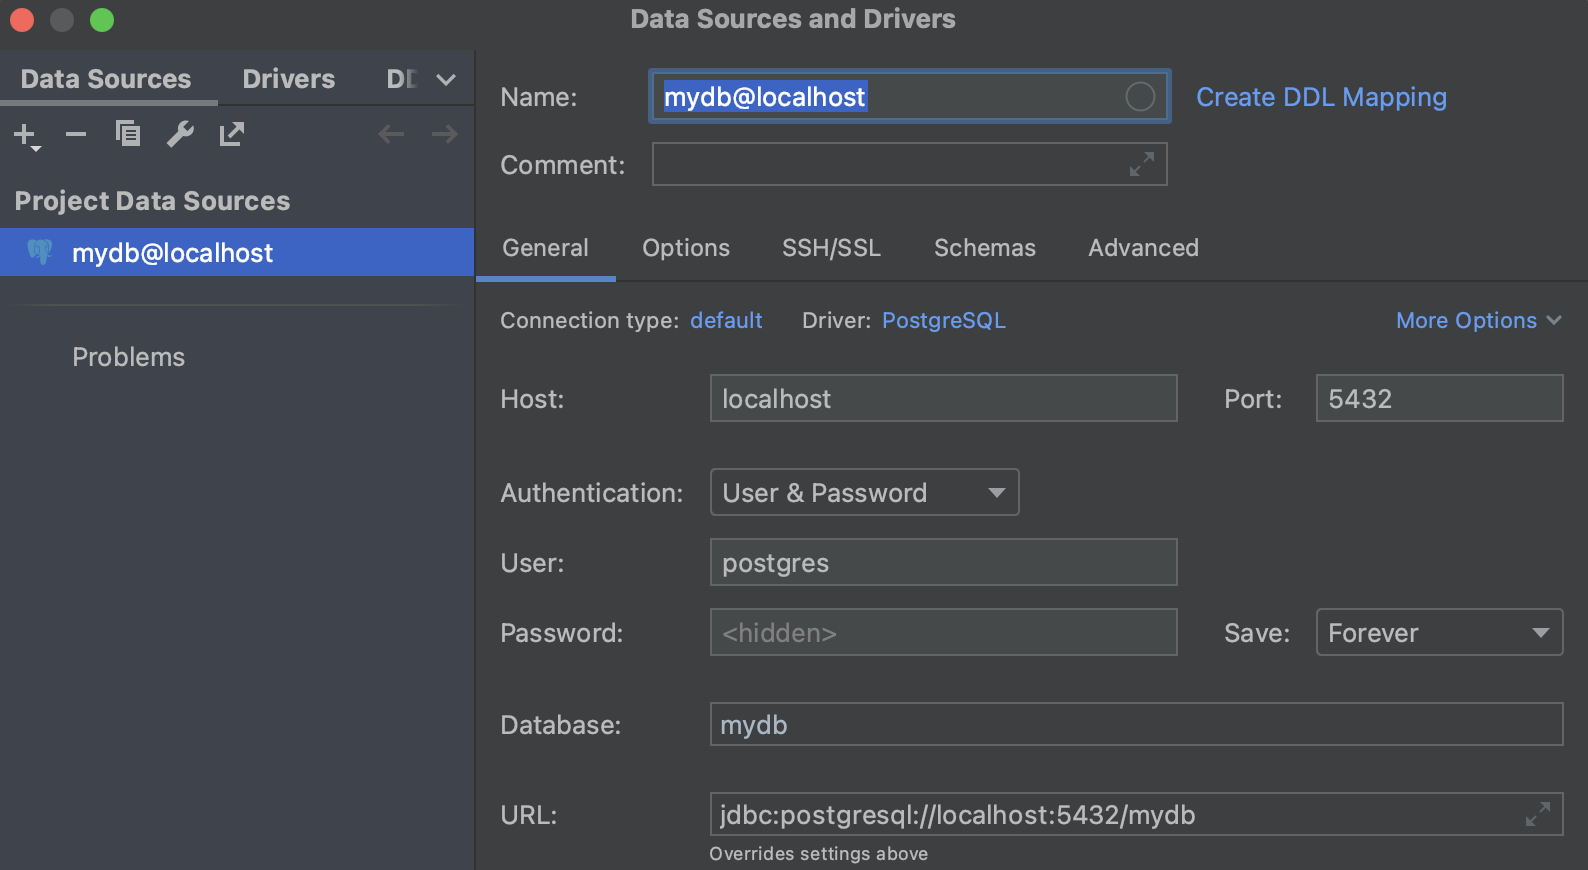
\includegraphics[width=.8\textwidth]{week4/config}

\end{frame}

\begin{frame}
点击「Test Connection」,出现下面的 \alert{Succeeded} 表明连接成功!

    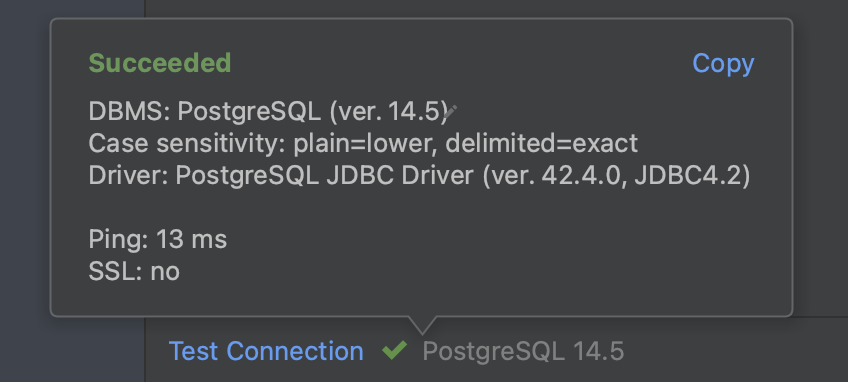
\includegraphics[width=.8\textwidth]{week4/connection} 

\end{frame}

\begin{frame}[fragile]

    \section{\textcolor{darkmidnightblue}{2. 导入数据}}
    \href{https://github.com/ChenZhongPu/db-swufe/tree/master/db-book}{db-book}:
    \begin{enumerate}
        \item DDL+drop.sql
        \item DDL.sql
        \item largeRelationsInsertFile.sql
        \item smallRelationsInsertFile.sql
    \end{enumerate}
\end{frame}

\begin{frame}
    \frametitle{2.1 导入 SQL}
    \begin{columns}
        \column{.4\textwidth}
        File $\rightarrow$ Open,选择 \alert{DDL.sql},打开右键菜单,选择「Run 'DDL.sql'」
        \column{.59\textwidth}
        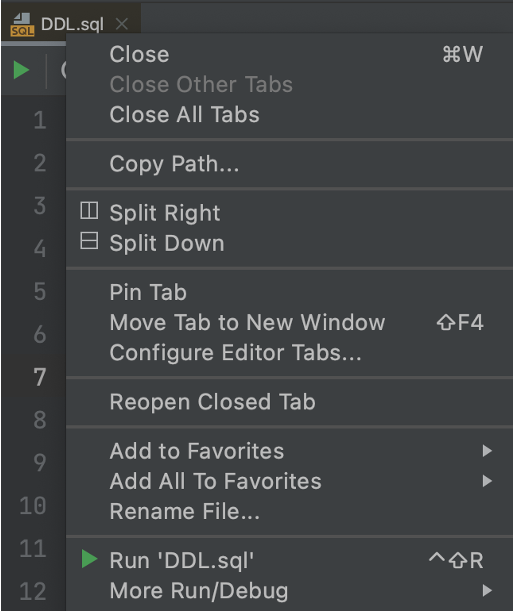
\includegraphics[height=.9\paperheight]{week4/ddl}  
    \end{columns}

\end{frame}

\begin{frame}
    \frametitle{2.2 配置数据源}
    点击下面的「public」,即选择了mydb.public为数据源:
    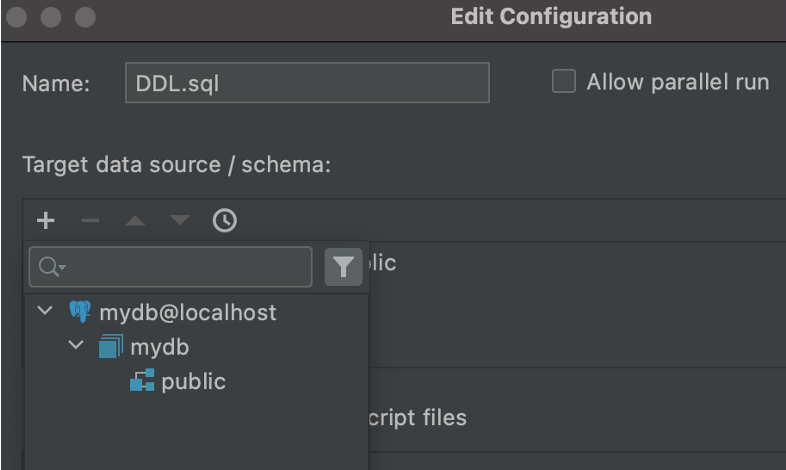
\includegraphics[height=.8\paperheight]{week4/public-source}  
\end{frame}

\begin{frame}
    \frametitle{2.3 运行结果}
    \begin{columns}
        \column{.45\textwidth}<1->
        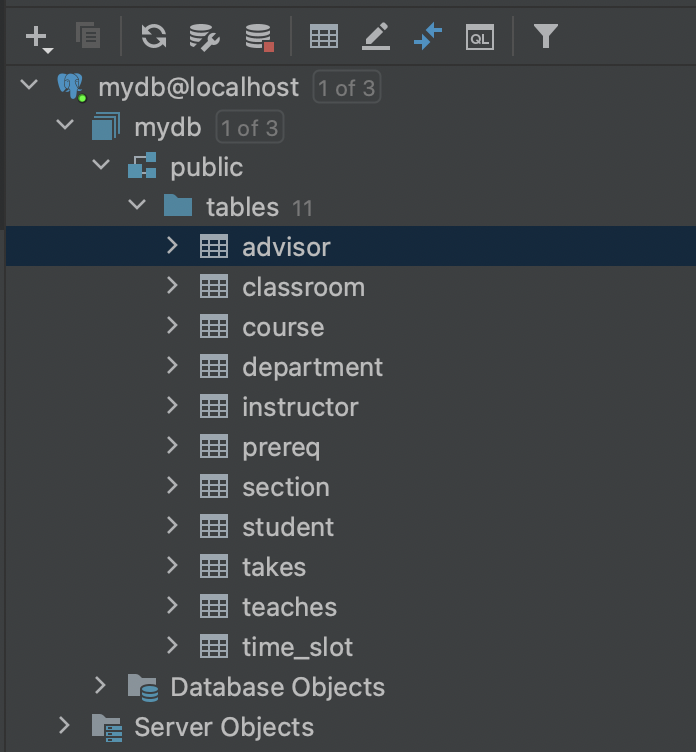
\includegraphics[height=.8\paperheight]{week4/result}   
        \column{.55\textwidth}<2->
        小任务
        \begin{enumerate}
            \item 阅读 DDL.sql 的内容
            \item 执行 smallRelationsInsertFile.sql 文件
        \end{enumerate}
    \end{columns}
\end{frame}

\begin{frame}

    \section{\textcolor{darkmidnightblue}{3. 编写 SQL}} 

\end{frame}

\begin{frame}
    \frametitle{3.1 新建 Query Console}
    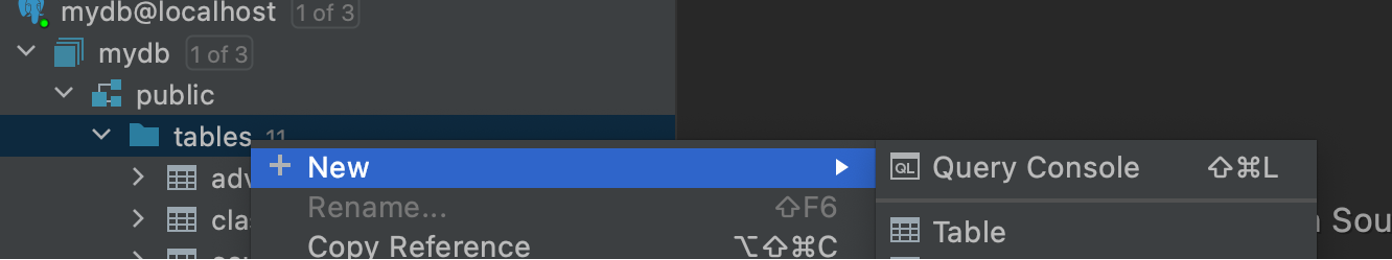
\includegraphics[height=.34\paperheight]{week4/console}  
    \pause
    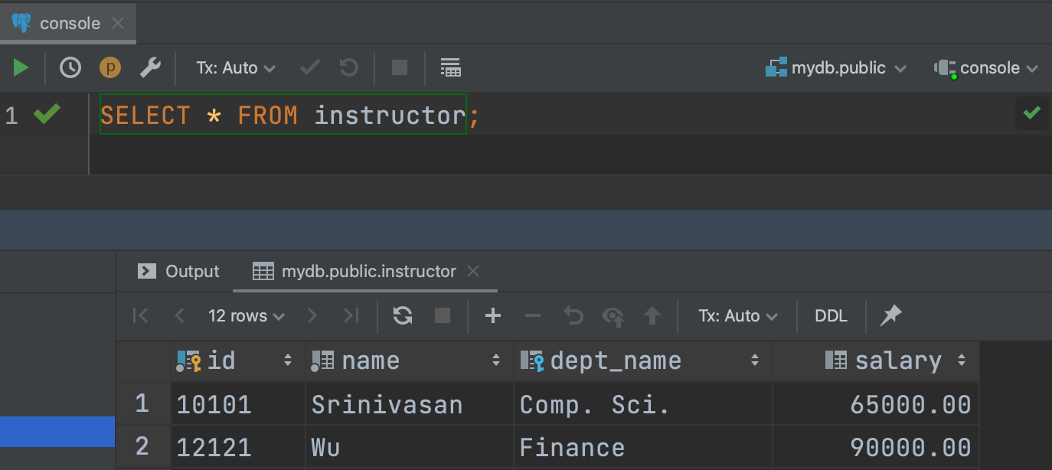
\includegraphics[height=.5\paperheight]{week4/select}   

\end{frame}

\begin{frame}[fragile]
\textbf{试试运行效果}:

\begin{minted}[bgcolor=LightGray]{sql} 
SELECT DISTINCT dept_name FROM instructor;       

SELECT name, salary / 12 FROM instructor;

SELECT name FROM instructor
WHERE dept_name = 'Physics';

SELECT name
FROM instructor
WHERE salary BETWEEN 90000 AND 100000;
\end{minted}      

\end{frame}

\begin{frame}
    \section{\textcolor{darkmidnightblue}{4. SQL 附加操作(续)}}  
更名、排序、\alert{字符串操作}
\end{frame}

\begin{frame}
    \frametitle{小测试}
{
    \renewcommand{\theenumi}{\Alph{enumi}}
    SQL 通过一对\_\_\_表示字符串。
    \begin{enumerate}
        \item 单双号
        \item 双引号
        \item 单双引号皆可
    \end{enumerate}
}        

\end{frame}

\begin{frame}
    \frametitle{4.1 引号问题}
\begin{itemize}
    \item<1-> 如果字符串里面本来就有单引号怎么办?
    
    \texttt{I'm good} $\rightarrow$ \texttt{I''m good}

    使用两个单引号表示即可。但注意\alert{两个单引号不等于一个双引号}!
    \item<2-> 如果字符串里面本来就有双引号怎么办?
    
    \texttt{I am "good"}

    不变!
\end{itemize}
    
\end{frame}

\begin{frame}[fragile]
    \begin{minted}[bgcolor=LightGray]{sql} 
SELECT 'I''m good. "Good"?'
    \end{minted}

    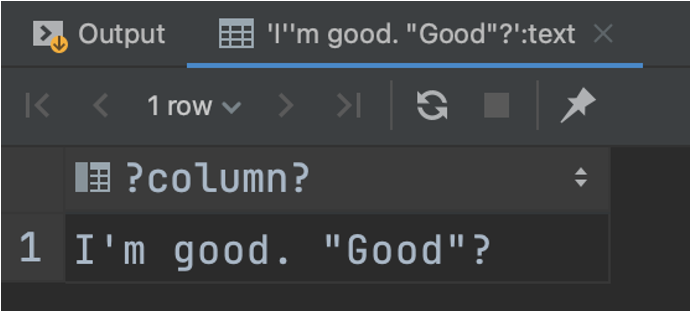
\includegraphics[height=.6\paperheight]{week4/good}    
\end{frame}

\begin{frame}[fragile]
    字符串在SQL标准中是区分大小写的,即 \texttt{china} 不等于 \texttt{CHINA}:
\begin{minted}[bgcolor=LightGray]{sql} 
/*
 MySQL 和 SQLServer 不区分, PG 区分
*/
SELECT 'china' = 'CHINA';
\end{minted}
    \pause
\noindent\rule{\textwidth}{1pt}
\textbf{布尔类型}(\texttt{boolean})
\begin{quote}
    The \texttt{boolean} type can have several states: \alert{true}, \alert{false}, and a third state, \alert{unknown}, which is represented by the SQL \alert{null} value.
\end{quote}

\end{frame}

\begin{frame}[fragile]
    \frametitle{4.2 字符串函数}

\begin{minted}[bgcolor=LightGray]{sql} 
SELECT lower('CHINA'), upper('good');

SELECT trim('   SWUFE ') = 'SWUFE';

SELECT lower(dept_name) FROM department;

SELECT dept_name, length(dept_name) FROM department;
\end{minted}

\end{frame}

\begin{frame}
    \frametitle{4.3 模糊查询}
    
\includegraphics[width=.8\textwidth]{week4/china.png}
\begin{columns}
    \column{.4\textwidth}<1->
    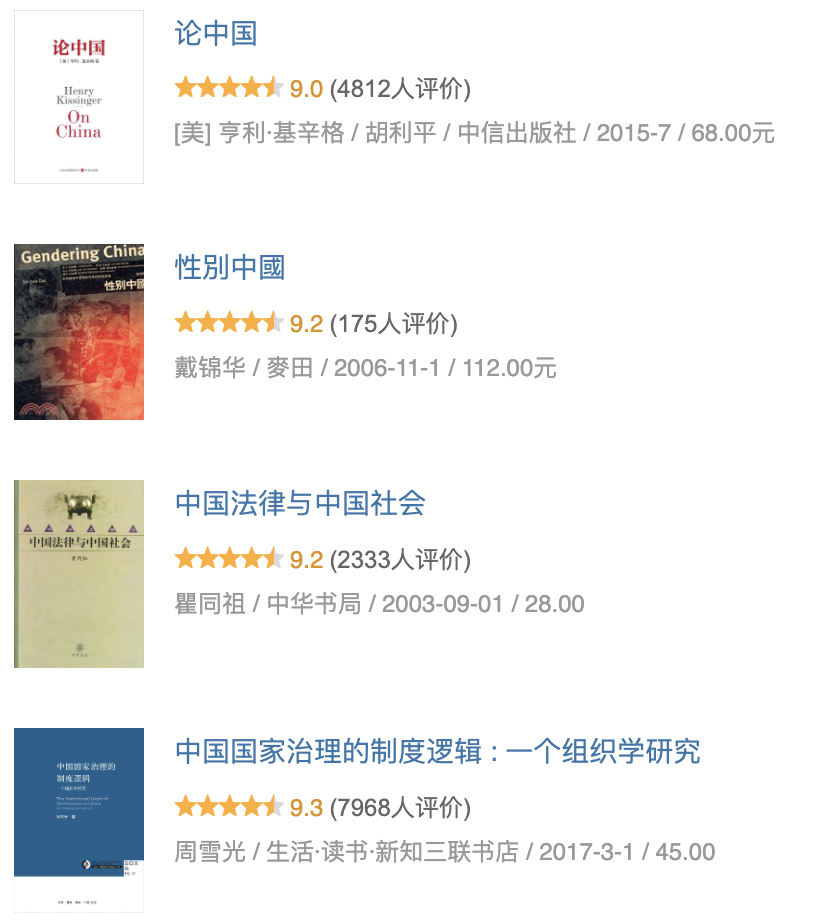
\includegraphics[height=.7\paperheight]{week4/china2.png} 
    \column{.6\textwidth}<2->
SQL 中使用 \alert{like} 操作符进行模式匹配(pattern matching):
\begin{itemize}
    \item \texttt{\%}:表示匹配任意字符串
    \item \texttt{\_}:表示匹配任意字符
\end{itemize}

\end{columns}

\end{frame}

\begin{frame}[fragile]
    \begin{minted}[bgcolor=LightGray]{sql} 
SELECT * FROM department
WHERE dept_name LIKE 'His%';

SELECT * FROM department
WHERE dept_name NOT LIKE '%sic%';
    \end{minted}
    \pause
    \noindent\rule{\textwidth}{1pt}
    {\large \faIcon{code}} \textbf{练习}:
\begin{itemize}
    \item \texttt{'abc' LIKE 'abc'}    
    \item \texttt{'abc' LIKE 'a\%'} 
    \item \texttt{'abc' LIKE '\_b\_'} 
    \item \texttt{'abc' LIKE 'c'}
\end{itemize}
\end{frame}


\begin{frame}[fragile]
    \frametitle{思考 (1)}

运行下面的语句,你有什么结论?关系 \texttt{instructor} 有个教师名字是 \texttt{Wu}:

\begin{minted}[bgcolor=LightGray]{sql} 
SELECT *
FROM instructor
WHERE name LIKE 'Wu%';

SELECT *
FROM instructor
WHERE name LIKE 'Wu_';
\end{minted}
    
\end{frame}

\begin{frame}[fragile]
    \frametitle{思考 (2)}

    \begin{columns}
        \column{.4\textwidth}
        \begin{table}
            \caption*{The \texttt{users} table}
            \begin{tabular}{ll}
              \toprule
              name & gender \\
              \midrule
              abc\%dd & m \\
              abcdd & f \\
              \bottomrule
            \end{tabular}
        \end{table}
        \column{.6\textwidth}
        {\large \faIcon[regular]{lightbulb}} 下面的 SQL 语句会输出几条结果?

        \begin{minted}[bgcolor=LightGray]{sql} 
SELECT *
FROM users
WHERE name LIKE 'abc%d%';
        \end{minted}
    \end{columns}



\end{frame}

\begin{frame}[fragile]
    \frametitle{4.4 转义字符}
如果要匹配\texttt{\%}本身,需要使用\alert{\textbackslash\%}。
\begin{minted}[bgcolor=LightGray]{sql} 
SELECT * FROM users
WHERE name LIKE 'abc\%d%';
\end{minted}
\begin{quote}
    当\alert{转义字符} (escape character) 放在字符序列时,它将对它后续的几个字符进行替代并解释。
\end{quote}

PG中默认的转义字符是反斜线\textbackslash,英文 backslash。
\end{frame}

\begin{frame}[fragile]
    \begin{minted}[bgcolor=LightGray]{python} 
# Python
s = 'database is \n very fun'
print(s)
    \end{minted}
    \pause
    \begin{table}
        \begin{tabular}{ll}
          \toprule
          name & gender \\
          \midrule
          abc\%dd & m \\
          abcdd & f \\
          ab\textbackslash nd & f \\
          \bottomrule
        \end{tabular}
    \end{table}
{\large \faIcon[regular]{lightbulb}} \textbf{思考}:如何匹配以 \texttt{ab\textbackslash n} 的 \texttt{name}?
\end{frame}

\begin{frame}[fragile]
    \frametitle{4.5 值的拼接}
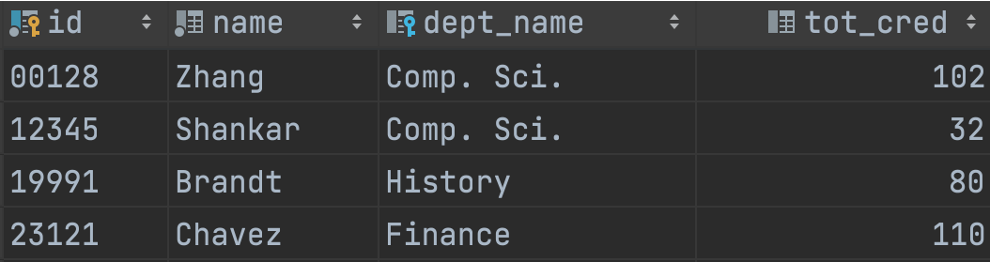
\includegraphics[width=.8\textwidth]{week4/cred}    

找到总学分大于 50 的学生,打印其信息,格式为

\begin{verbatim}
{name} from {dept_name}    
\end{verbatim}

比如,\texttt{Zhang from Compu. Sci.}。
\end{frame}

\begin{frame}[fragile]
PG 使用 \alert{||} 进行拼接:
    \begin{minted}[bgcolor=LightGray]{sql} 
/*
SQLServer 用 +
MySQL用 concat 函数
*/
SELECT name || 'from' || dept_name
FROM student
WHERE tot_cred > 50;
    \end{minted}

\end{frame}

\begin{frame}[fragile]
    \frametitle{资源}
PG 中的字符串操作异常丰富,可以参考 \href{https://www.postgresql.org/docs/14/functions-string.html}{String Functions and Operators} 和 \href{https://www.postgresql.org/docs/14/functions-matching.html}{Pattern Matching}。

\begin{minted}[bgcolor=LightGray]{sql} 
SELECT * FROM instructor
WHERE name ~~ 'Z%';

SELECT * FROM instructor
WHERE name SIMILAR TO '(Z|Y)%';

SELECT substr(name, 2) FROM instructor;
\end{minted}

\end{frame}

\begin{frame}
    \section{\textcolor{darkmidnightblue}{5. SQL 集合操作}}  
并、交、差    
\end{frame}

\begin{frame}[fragile]
    \frametitle{5.1 并}
所有在 2017 年 Fall 学期或 2018 年 Spring 学期或者在这两学期都开的课程。

\begin{minted}[bgcolor=LightGray]{sql}
(SELECT course_id
FROM section
WHERE semester = 'Fall' AND year = 2017)
UNION
(SELECT course_id
FROM section
WHERE semester = 'Spring' AND year = 2018);
\end{minted}
    
\end{frame}

\begin{frame}[fragile]
\frametitle{5.2 交}
    \begin{minted}[bgcolor=LightGray]{sql}
/*
MySQL does not support intersect
*/
(SELECT course_id
FROM section
WHERE semester = 'Fall' AND year = 2017)
INTERSECT
(SELECT course_id
FROM section
WHERE semester = 'Spring' AND year = 2018);
    \end{minted} 

\end{frame}

\begin{frame}[fragile]
    \frametitle{5.3 差}

    \begin{minted}[bgcolor=LightGray, baselinestretch=1]{sql}
/*
MySQL does not support except.
Oracle use the keyword minus in place of except.
*/
(SELECT course_id
FROM section
WHERE semester = 'Fall' AND year = 2017)
EXCEPT
(SELECT course_id
FROM section
WHERE semester = 'Spring' AND year = 2018);
    \end{minted}     

\end{frame}

% \begin{frame}
%     \section{\textcolor{darkmidnightblue}{6. DDL 补充}}  
%     \texttt{CREATE TABLE}、\texttt{DROP TABLE}、\alert{\texttt{ALTER TABLE}}

% \end{frame}

% \begin{frame}[fragile]
%     \frametitle{6.1 添加属性}
% \begin{minted}[bgcolor=LightGray]{sql}
% ALTER TABLE r ADD COLUMN a d
% \end{minted}
% \pause
% 为 student 添加新的属性 nationality

% \begin{minted}[bgcolor=LightGray]{sql}
% ALTER TABLE student
% ADD COLUMN nationality varchar(20);
% \end{minted}
% \end{frame}

% \begin{frame}[fragile]
%     \frametitle{6.2 删除属性}
% \begin{minted}[bgcolor=LightGray]{sql}
% ALTER TABLE r DROP COLUMN a;
% \end{minted}

% 为 student 删除属性 nationality

%     \begin{minted}[bgcolor=LightGray]{sql}
% ALTER TABLE student
% DROP COLUMN nationality;
%     \end{minted}

% \end{frame}

% \begin{frame}[fragile]
%     \begin{minted}[bgcolor=LightGray]{sql}
% CREATE TABLE products (
%     product_no integer,
%     name text,
%     price numeric -- PG 中 numeric 表示机器上限的精度
% );
%     \end{minted}
    
% \end{frame}

% \begin{frame}
%     \frametitle{6.3 修改属性的类型}
% \end{frame}

\begin{frame}
    \section{\textcolor{darkmidnightblue}{总结}}   
    \begin{enumerate}
        \item 连接数据库,执行 SQL 文件
        \item 字符串相关操作
        \item 集合操作
    \end{enumerate}

\end{frame}

\begin{frame}
    \frametitle{Homework 3}

    \href{https://github.com/ChenZhongPu/db-swufe/tree/master/04_lab_sql}{04. Lab SQL}

\end{frame}

\begin{frame}
    \frametitle{case 表达式}

    考虑关系模式 marks(id, score),并规定如果 score < 60 等级为 C,60 $\leq$ score < 80 等级为 B,score $\geq$ 80 等级为 A。

    {\large \faIcon{question-circle}} \textbf{问题}:基于 marks 关系,显示每个学生的成绩等级。
    
\[
output = \begin{cases}
    A, & \text{if $score \geq 80$}; \\
    B, & \text{if $80 > score \geq 60$}; \\
    C, & \text{if $score < 60$}.
\end{cases}
\]
\end{frame}
\begin{frame}[fragile]
    \begin{minted}[bgcolor=LightGray, baselinestretch=.9]{sql}
CASE
    WHEN condition1 THEN result1
    WHEN condition2 THEN result2
    WHEN conditionN THEN resultN
    ELSE result
END;
    \end{minted}

    \begin{minted}[bgcolor=LightGray, baselinestretch=1]{sql}
SELECT ID,
    CASE
        WHEN score < 60 THEN 'C'
        WHEN score >= 80 THEN 'A'
        ELSE 'B'
    END
FROM marks;
    \end{minted}

\end{frame}

\end{document}